%Author: Steven Munn
%UCSB ECE 594

\documentclass[11pt, english]{article}

\usepackage{seqsplit}
\usepackage{listings}
\usepackage[T1]{fontenc}
\usepackage[latin9]{inputenc}
\usepackage[letterpaper]{geometry}
\usepackage{wrapfig}
\usepackage{graphicx}
\usepackage{caption}
\usepackage{subcaption}
\usepackage{babel}
\usepackage{amstext}
\usepackage{amsmath}
\usepackage{hyperref}
\usepackage{units}
\usepackage{algorithmicx}
\usepackage{algpseudocode}
\usepackage{amssymb}
\usepackage[ampersand]{easylist}

\usepackage{listings}
\usepackage{color}

\definecolor{dkgreen}{rgb}{0,0.6,0}
\definecolor{gray}{rgb}{0.5,0.5,0.5}
\definecolor{mauve}{rgb}{0.58,0,0.82}

\ListProperties(Hide=100, Hang=true, Progressive=3ex, Style*=$\bullet$ ,
Style2*=$\Rightarrow$)
\lstset{frame=tb,
  language=matlab,
  aboveskip=3mm,
  belowskip=3mm,
  showstringspaces=false,
  columns=flexible,
  basicstyle={\small\ttfamily},
  numbers=none,
  numberstyle=\tiny\color{gray},
  keywordstyle=\color{blue},
  commentstyle=\color{dkgreen},
  stringstyle=\color{mauve},
  breaklines=true,
  breakatwhitespace=true
  tabsize=0
}

\geometry{verbose,tmargin=1in,bmargin=1in,lmargin=1in,rmargin=1in}

\setlength{\parskip}{\smallskipamount}
\setlength{\parindent}{0pt}
\setlength{\parindent}{0.25in}

\newcommand{\tab}{\hspace*{2em}}
%\newcommand{\unit}[1]{\ensuremath{\, \mathrm{#1}}}
\newcommand{\btheta}{\boldsymbol{\theta}}
\newcommand{\p}[1]{\left(#1\right)}
%END HEADERS

\begin{document}

\title{ECE 594E: Homework 5}

\author{Steven Munn}

\date{Wednesday, May 27, 2015}

\maketitle

\section{Particle Filter for non-linear system}
\subsection{}

We plot two sample trajectories in figures \ref{st1} and \ref{st2}.

\begin{figure}[h]
  
  \centering
    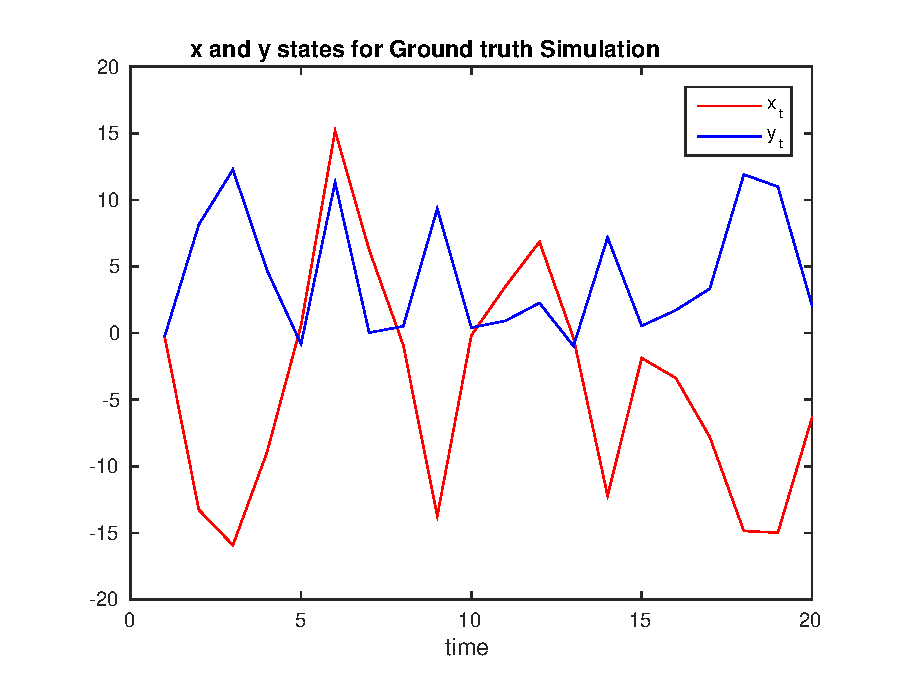
\includegraphics[width=80mm]{./figs/001_11_sampletraj1.eps}
    \caption{First sample trajectory}
    \label{st1}
\end{figure}

\begin{figure}[h]
  
  \centering
    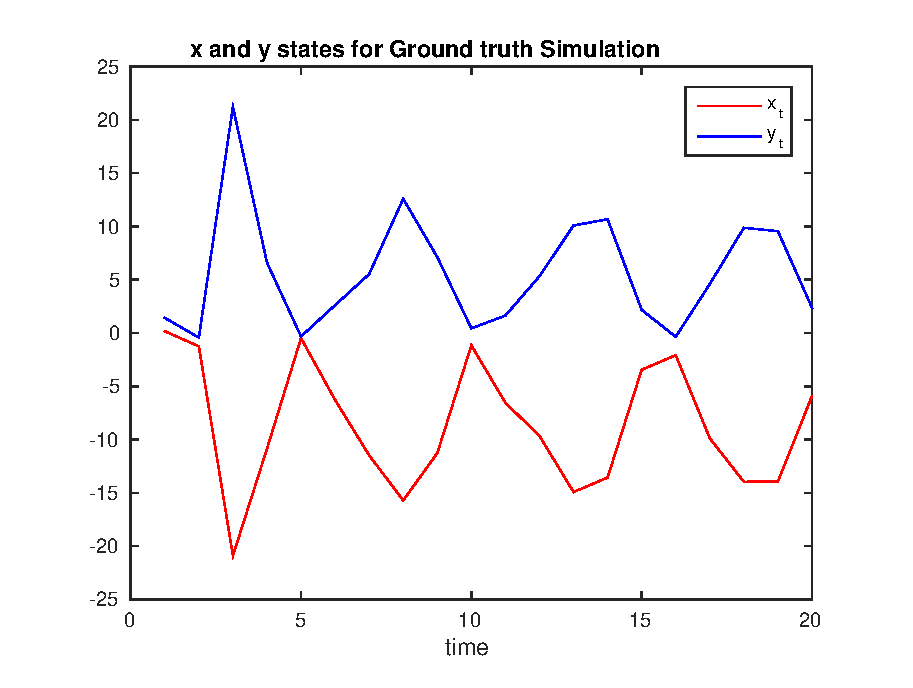
\includegraphics[width=80mm]{./figs/002_11_sampletraj2.eps}
    \caption{Second sample trajectory}
    \label{st2}
\end{figure}

\subsection{}

The full implementation code can be found at \url{https://github.com/stevenjlm/ML-code/tree/master/bootstrap}

\subsection{}

For $N=100$ particles, using measurements $y_t$, $t=1$ to $t=T=100$ we plot the conditional mean and the actual state in figure \ref{bs}. The mean square error between estimate and actual state is in figure \ref{mse}.

In figures \ref{t10}, \ref{t50}, and \ref{t100} we plot $p(x_{t}|y_{1:t})$ at times 10, 50, and 100. Only the plot at time 100 is bimodal, this mostly coincidence though. You can see in figure \ref{t50} that the peak is very close to zero. The distribution is a mixture of two Gaussians, it's just that their means are too close to produce distinguishable peaks. And, for figure \ref{t10} the value is so extremely low that the state must have been in a downward slope already and the step function didn't produce particles at the other mode peak.

\begin{figure}[h]
  
  \centering
    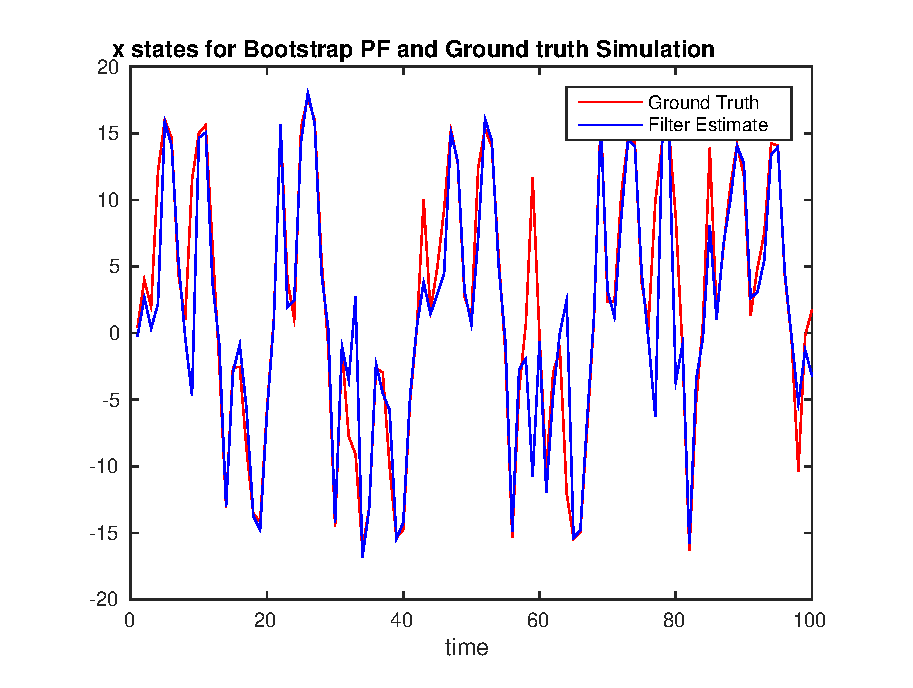
\includegraphics[width=80mm]{./figs/003_13_gt-and-bt.eps}
    \caption{Particle Filter estimate and actual state}
    \label{bs}
\end{figure}

\begin{figure}[h]
  
  \centering
    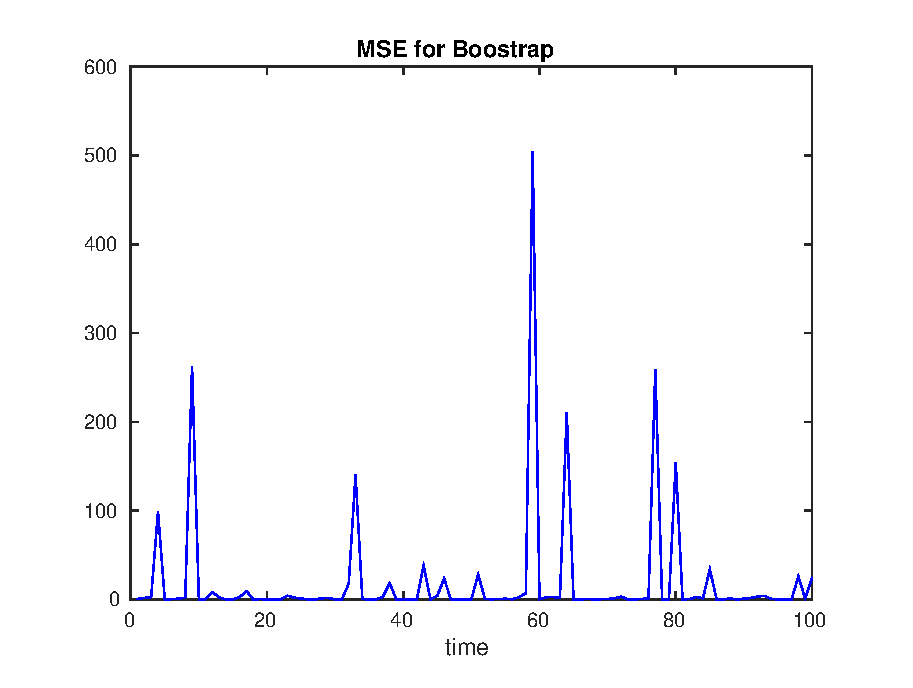
\includegraphics[width=80mm]{./figs/004_13_mse.eps}
    \caption{Mean square error of estimate}
    \label{mse}
\end{figure}

\begin{figure}[h]
  
  \centering
    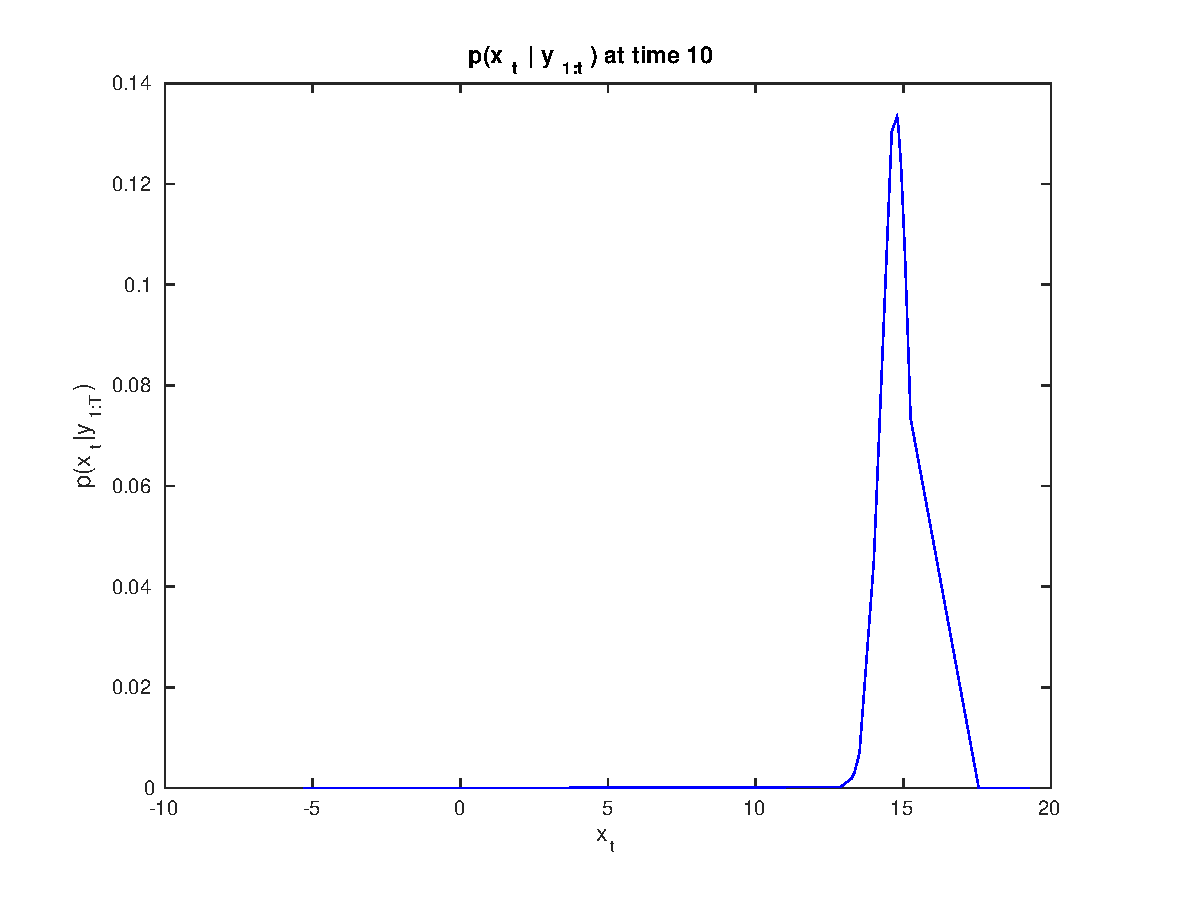
\includegraphics[width=80mm]{./figs/005_13_t10.eps}
    \caption{Filtering density at $t=10$ and $N=100$}
    \label{t10}
\end{figure}

\begin{figure}[h]
  
  \centering
    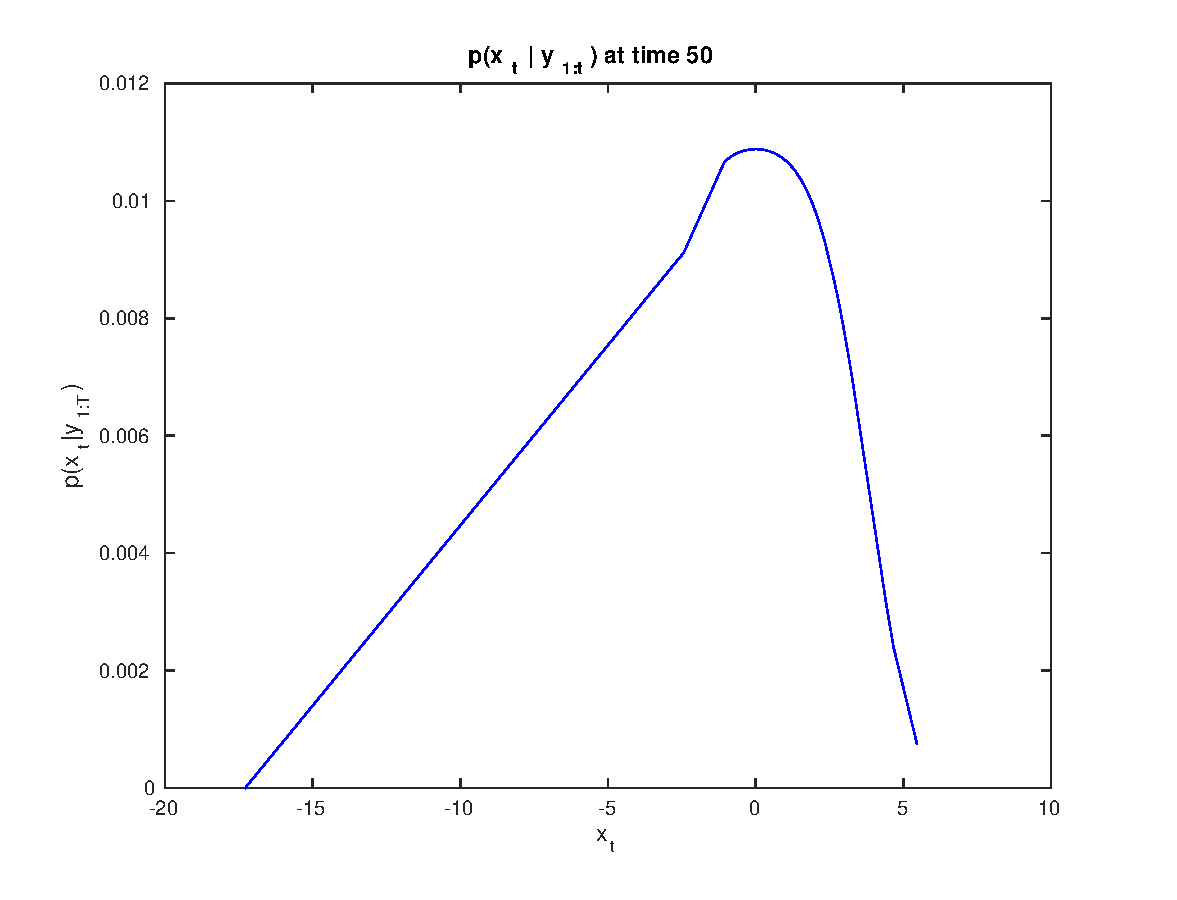
\includegraphics[width=80mm]{./figs/006_13_t50.eps}
    \caption{Filtering density at $t=50$ and $N=100$}
    \label{t50}
\end{figure}

\begin{figure}[h]
  
  \centering
    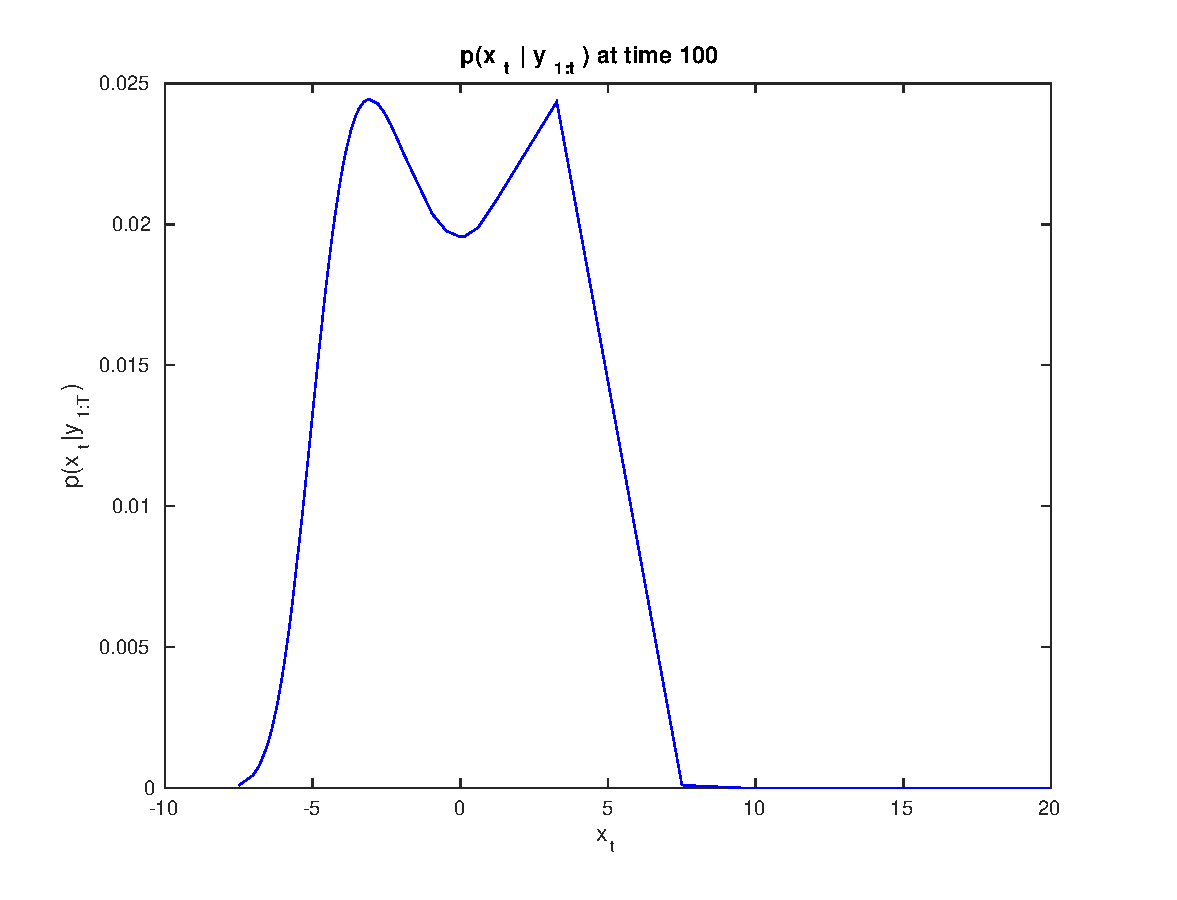
\includegraphics[width=80mm]{./figs/007_13_t100.eps}
    \caption{Filtering density at $t=100$ and $N=100$}
    \label{t100}
\end{figure}

\subsection{}

For $N=10$ we have the same plots as above in figures \ref{n10gtbt}, \ref{n10gtbt}, \ref{n101}, \ref{n102}, \ref{n103}, and \ref{n104}.

\begin{figure}[h]
  
  \centering
    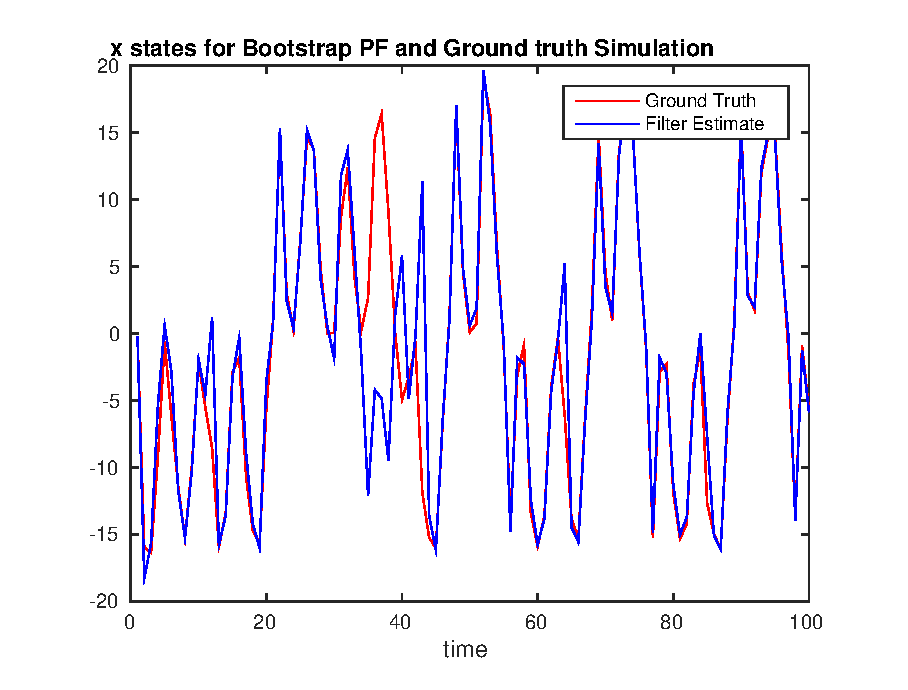
\includegraphics[width=80mm]{./figs/008_15_gt-and-bt.eps}
    \caption{Particle Filter estimate and actual state}
    \label{n10gtbt}
\end{figure}

\begin{figure}[h]
  
  \centering
    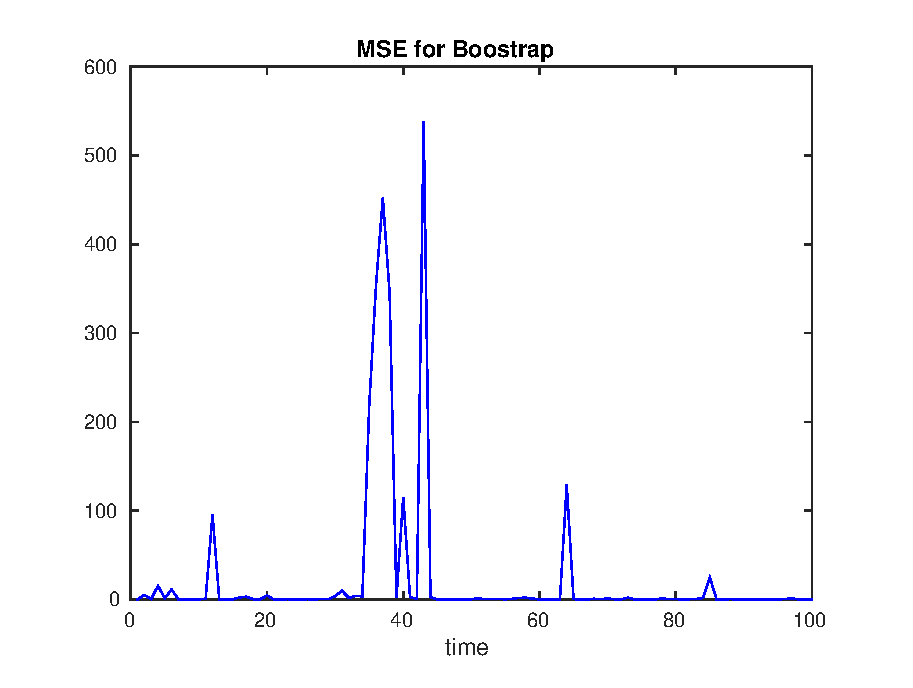
\includegraphics[width=80mm]{./figs/009_13_mse.eps}
    \caption{Mean square error of estimate}
    \label{n101}
\end{figure}

\begin{figure}[h]
  
  \centering
    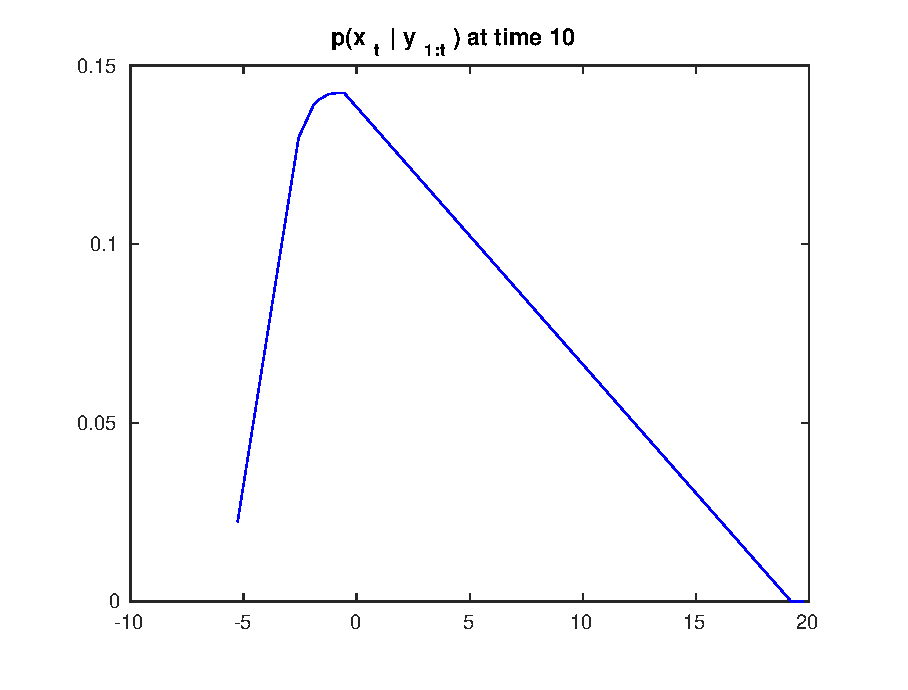
\includegraphics[width=80mm]{./figs/010_15_t10N10.eps}
    \caption{Filtering density at $t=10$ and $N=10$}
    \label{n102}
\end{figure}

\begin{figure}[h]
  
  \centering
    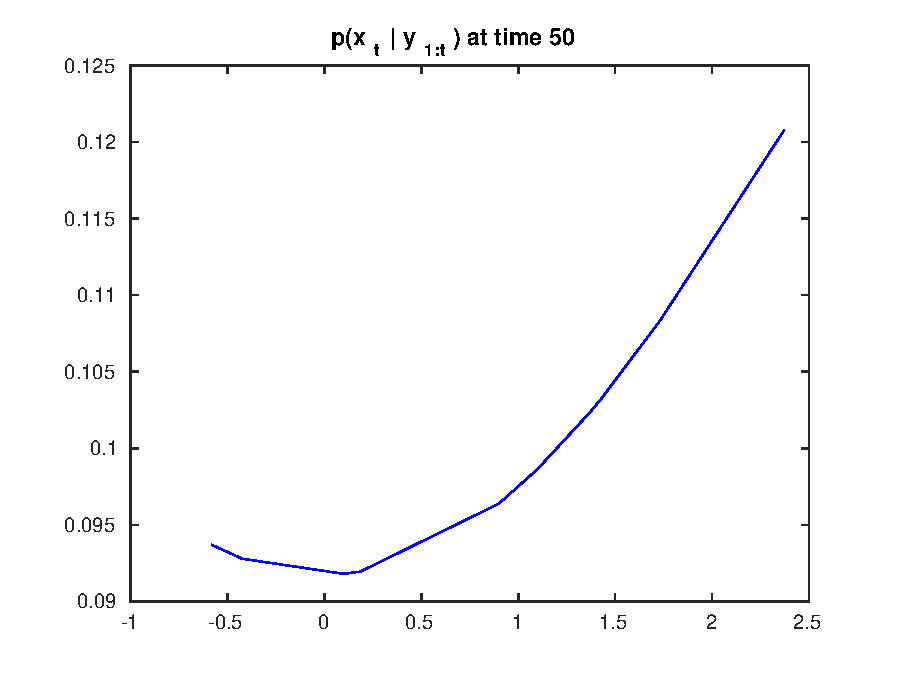
\includegraphics[width=80mm]{./figs/011_15_t50N10.eps}
    \caption{Filtering density at $t=50$ and $N=10$}
    \label{n103}
\end{figure}

\begin{figure}[h]
  
  \centering
    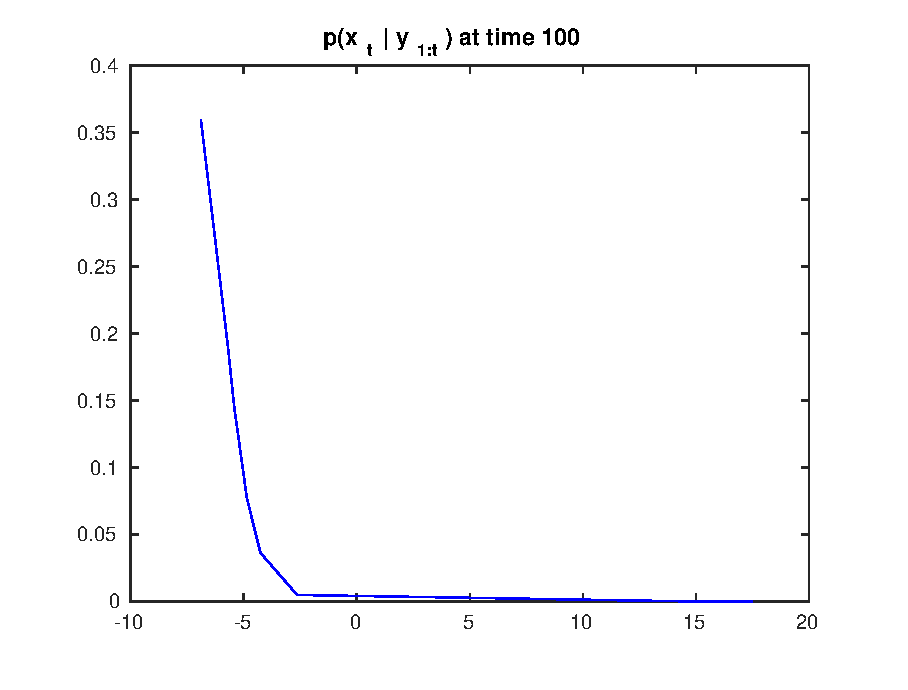
\includegraphics[width=80mm]{./figs/012_15_t100N10.eps}
    \caption{Filtering density at $t=100$ and $N=10$}
    \label{n104}
\end{figure}


For $N=1000$ we have the same plots as above in figures \ref{n1000gtbt}, \ref{n1000gtbt}, \ref{n10001}, \ref{n10002}, \ref{n10003}, and \ref{n10004}.

\begin{figure}[h]
  
  \centering
    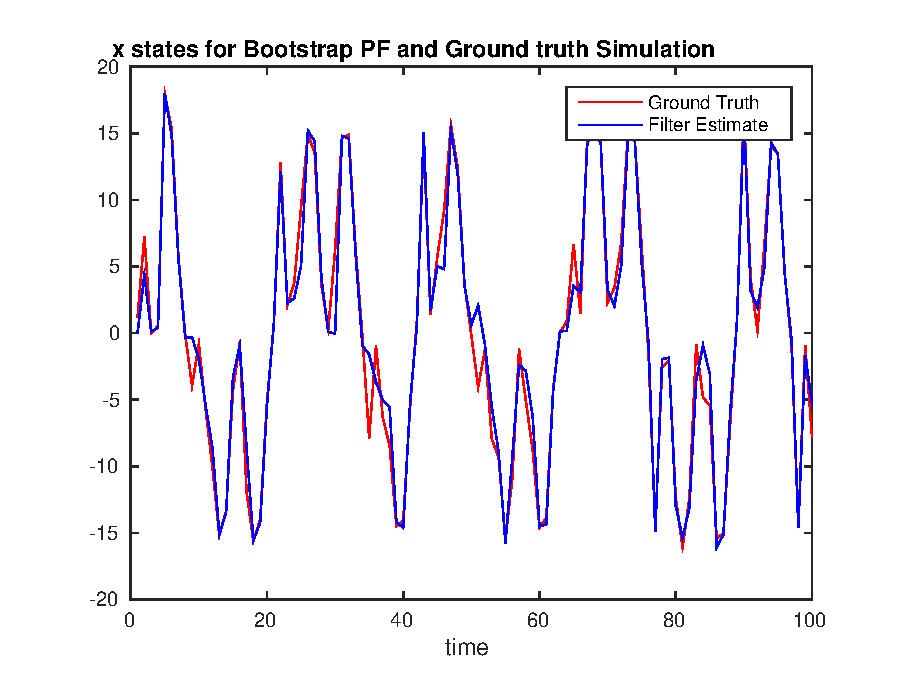
\includegraphics[width=80mm]{./figs/013_15_gt-and-bt.eps}
    \caption{Particle Filter estimate and actual state}
    \label{n1000gtbt}
\end{figure}

\begin{figure}[h]
  
  \centering
    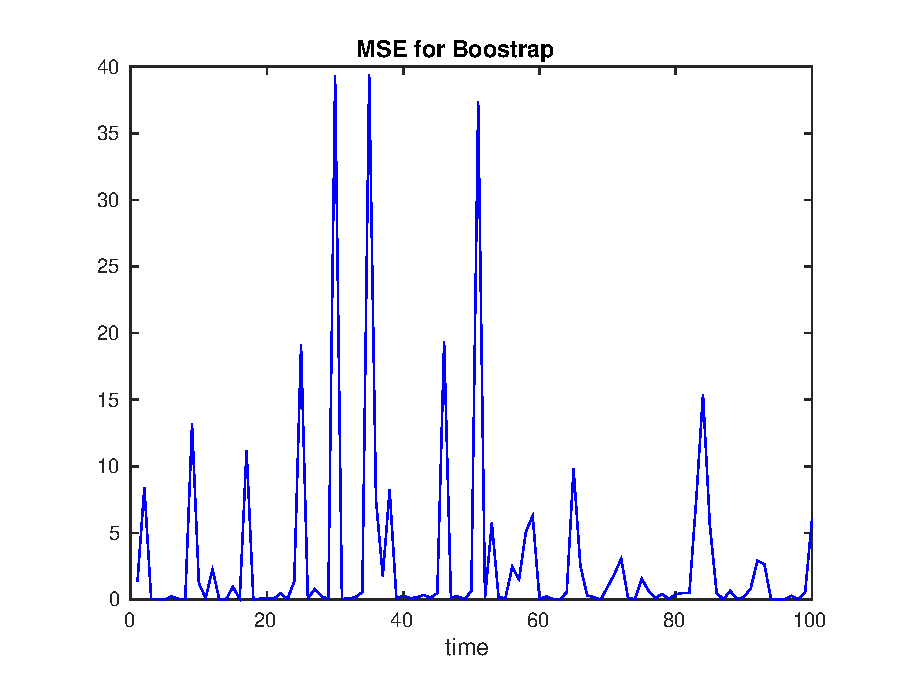
\includegraphics[width=80mm]{./figs/014_15_mseN1000.eps}
    \caption{Mean square error of estimate}
    \label{n10001}
\end{figure}

\begin{figure}[h]
  
  \centering
    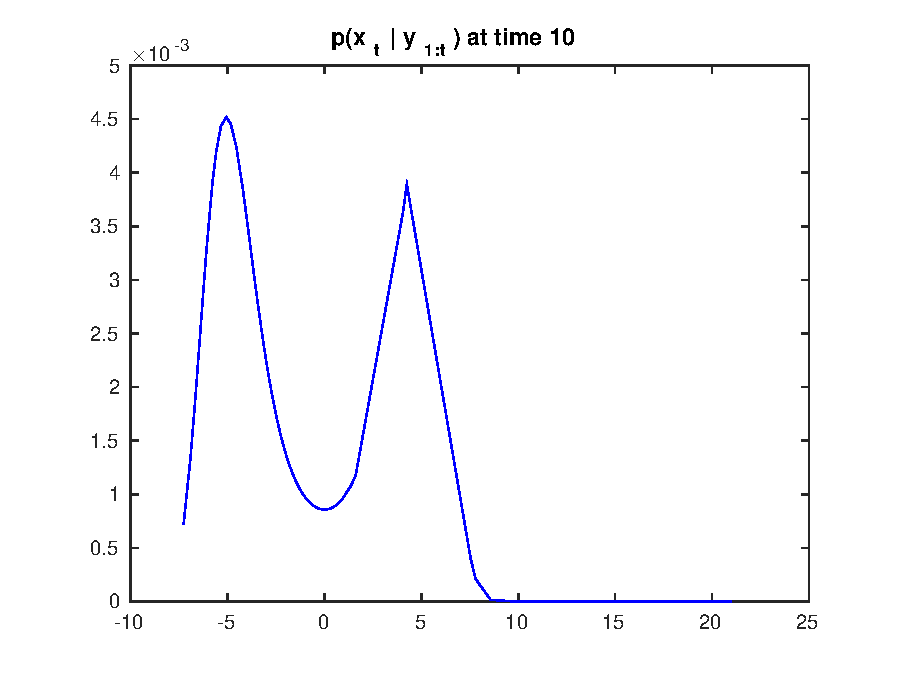
\includegraphics[width=80mm]{./figs/015_15_t10N1000.eps}
    \caption{Filtering density at $t=10$}
    \label{n10002}
\end{figure}

\begin{figure}[h]
  
  \centering
    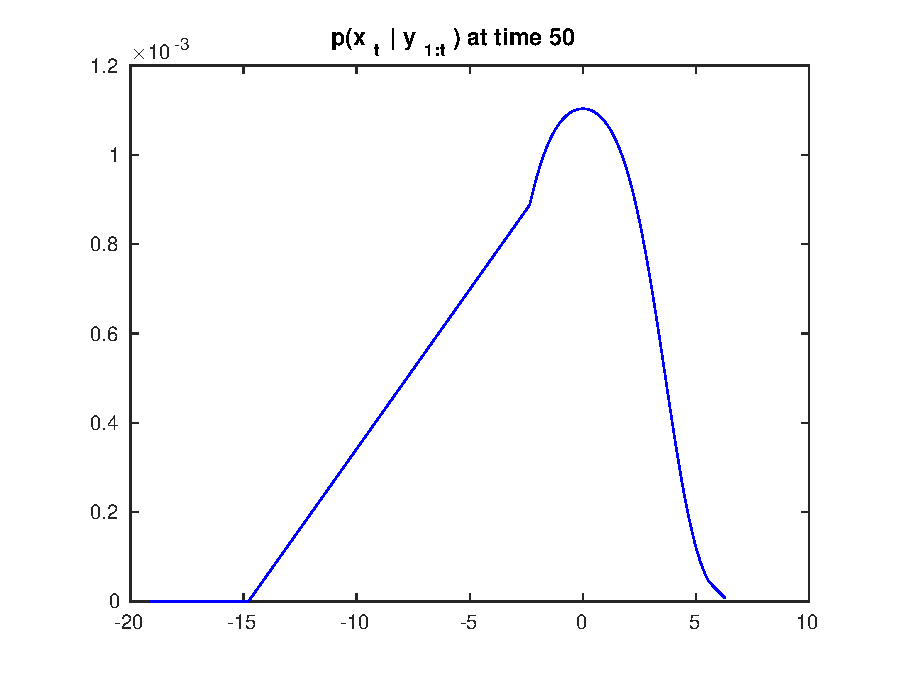
\includegraphics[width=80mm]{./figs/016_15_t50N1000.eps}
    \caption{Filtering density at $t=50$}
    \label{n10003}
\end{figure}

\begin{figure}[h]
  
  \centering
    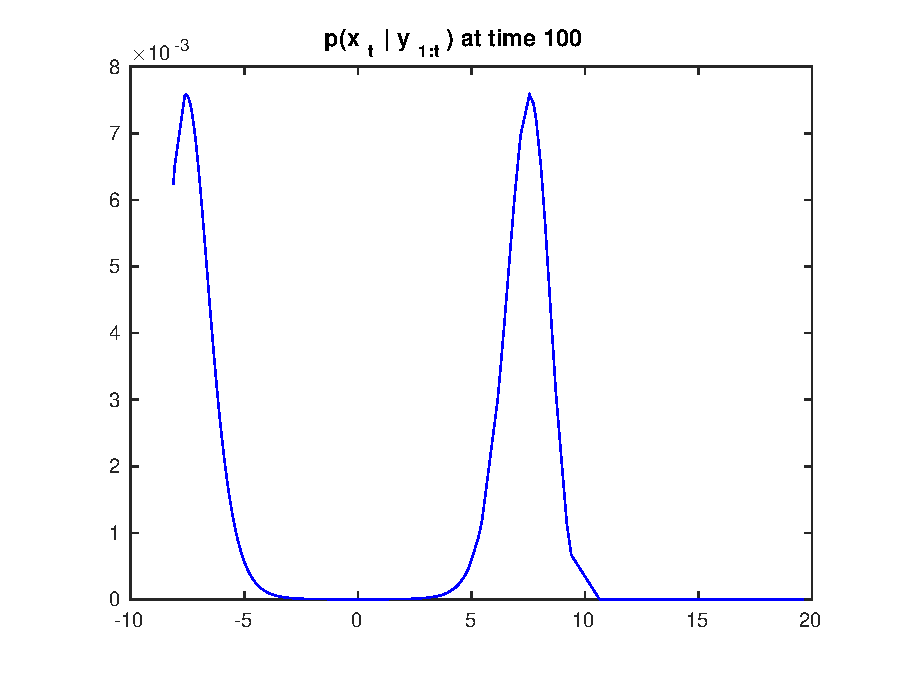
\includegraphics[width=80mm]{./figs/017_15_t100N1000.eps}
    \caption{Filtering density at $t=100$}
    \label{n10004}
\end{figure}

\subsection{}

Backward filter is implemented in the same runme.m file as the bootstrap filter. Figure \ref{bk} shows the actual state and some sample backward trajectories.

\begin{figure}[h]
  
  \centering
    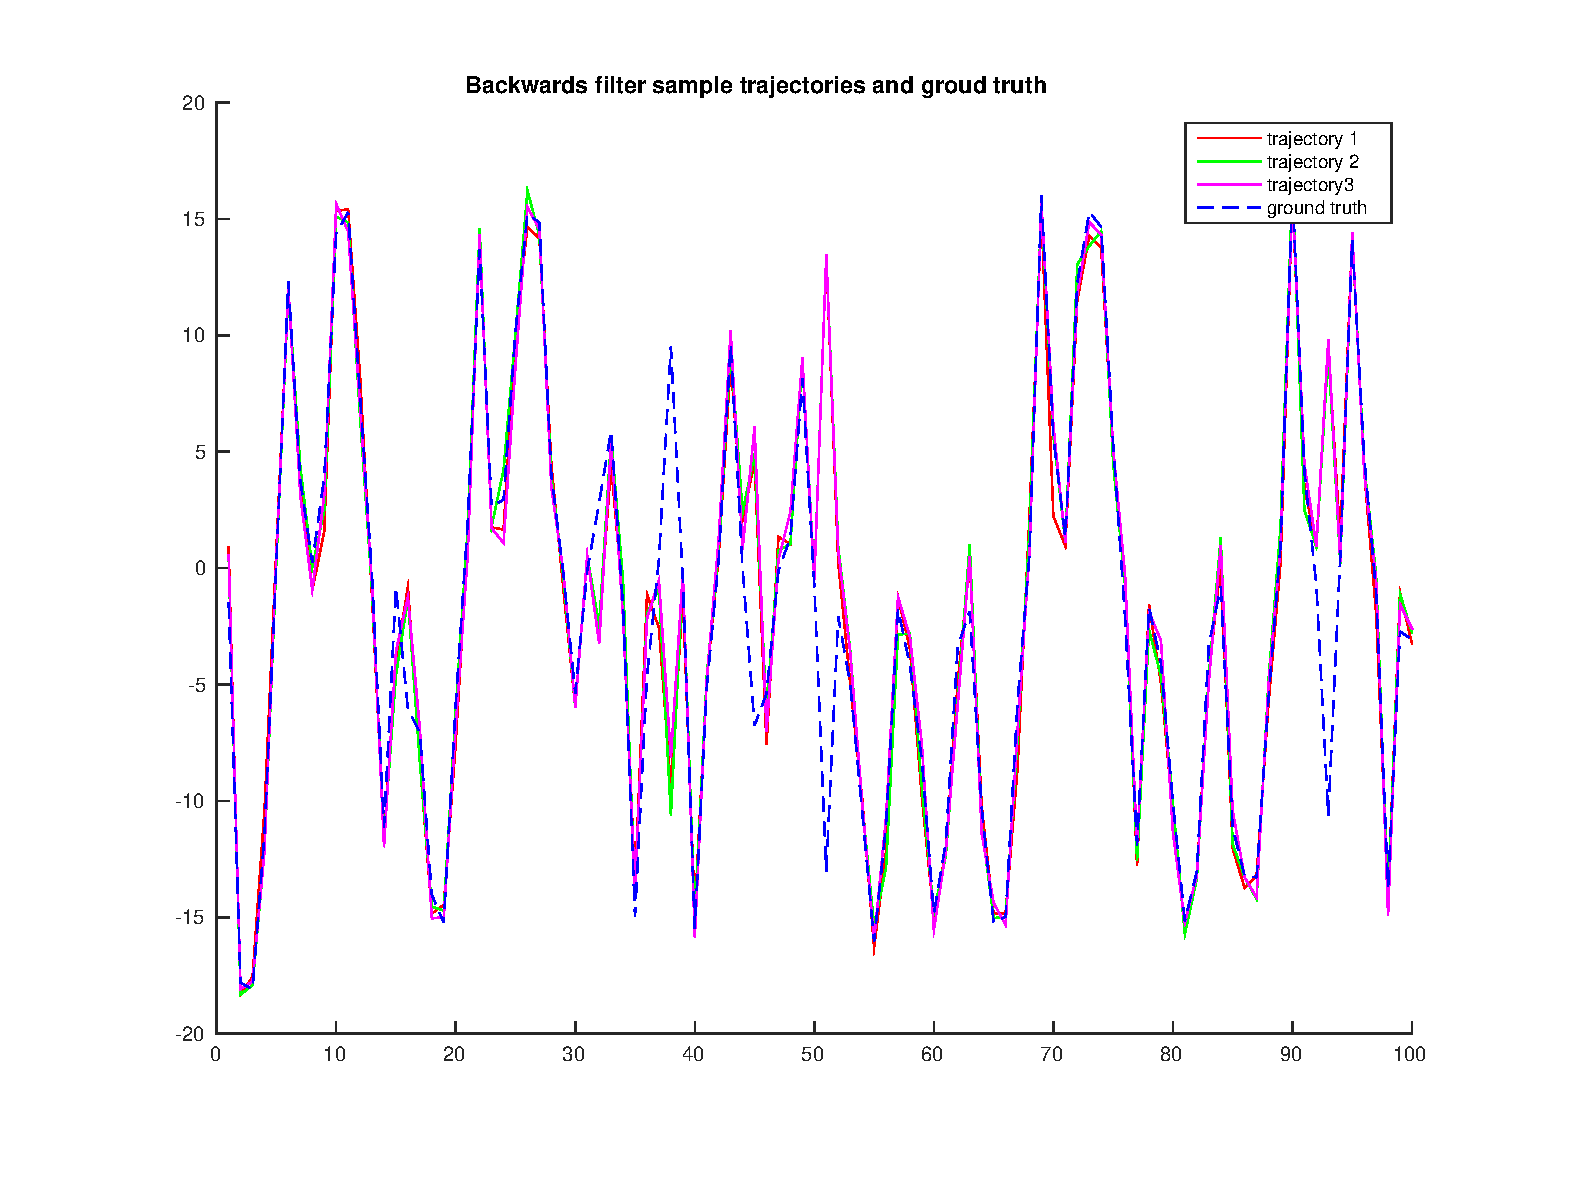
\includegraphics[width=80mm]{./figs/018_16bksam.eps}
    \caption{Backwards Filtering sample trajectories and actual trajectory.}
    \label{bk}
\end{figure}

\subsection{}

The mean square error over the average of forward filtered particles is 0.3012 and the backward filter gets 0.2561.

\subsection{}

With $N=10$ backward particles, the MSE is hardly any better after backward filtering. With $N=100$ particles however, the MSE is significantly better since it goes down nearly one third.

\section{Kalman Filtering}

\subsection{}

The full implementation code can be found at \url{https://github.com/stevenjlm/ML-code/tree/master/kalman}

\subsection{}

Figures \ref{bk}, \ref{k1}, \ref{k2}, and \ref{k3} show the various mean square errors for different values of N. $N=5000$ seems to be the point at which bootstrap becomes more acceptable; however, the Kalman filter is always the best.

\begin{figure}[h]
  
  \centering
    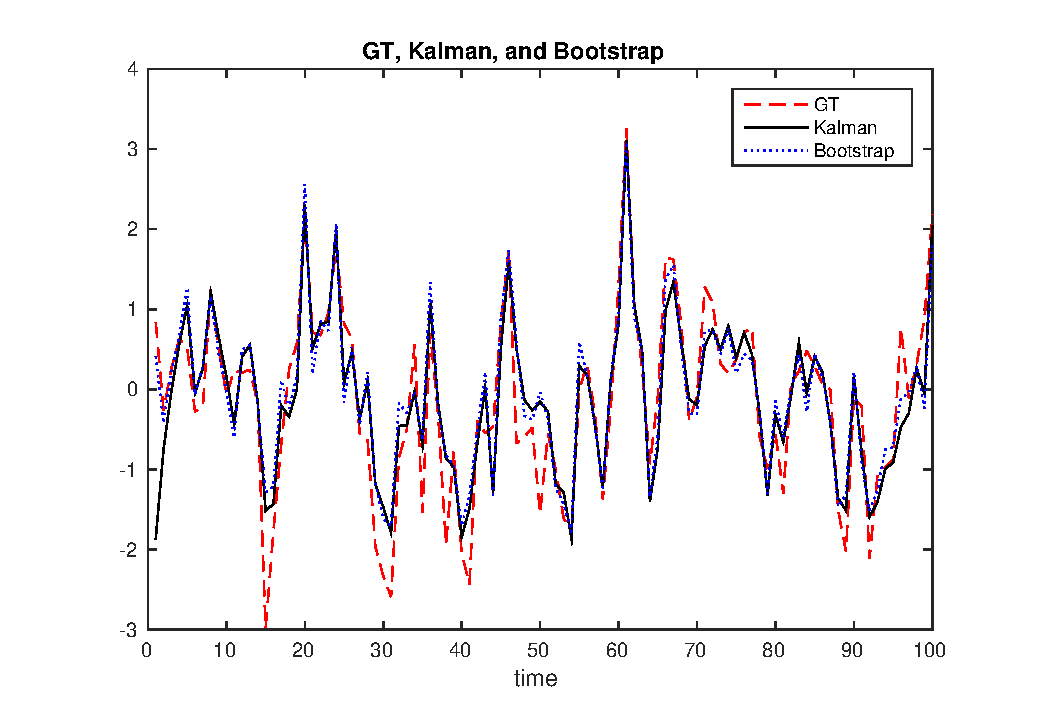
\includegraphics[width=80mm]{./kfigs/001_a3.eps}
    \caption{Sample trajectory ground truth, Kalman filter trajectory, and Bootstrap particle filter mean trajectories}
    \label{bk}
\end{figure}

\begin{figure}[h]
  
  \centering
    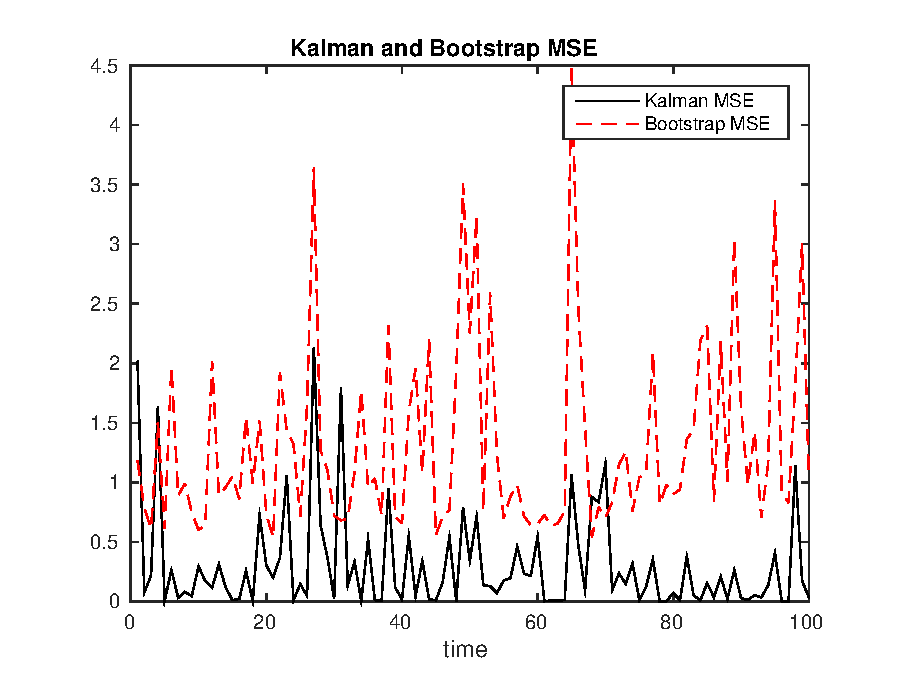
\includegraphics[width=80mm]{./kfigs/002_n100MSE.eps}
    \caption{Mean square error for $N=100$}
    \label{k1}
\end{figure}

\begin{figure}[h]
  
  \centering
    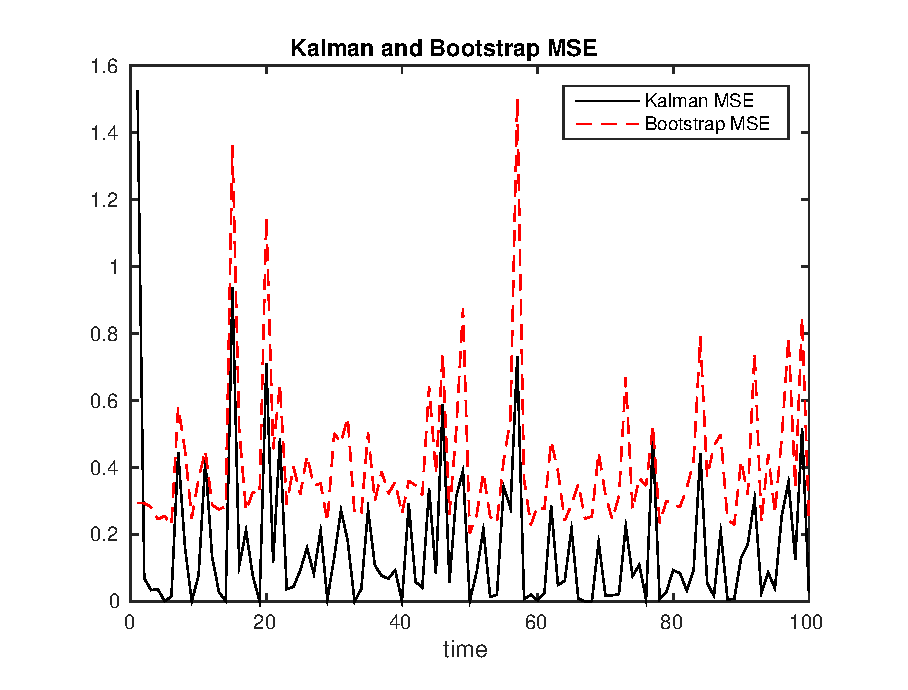
\includegraphics[width=80mm]{./kfigs/003_n1000MSE.eps}
    \caption{Mean square error for $N=1000$}
    \label{k2}
\end{figure}

\begin{figure}[h]
  
  \centering
    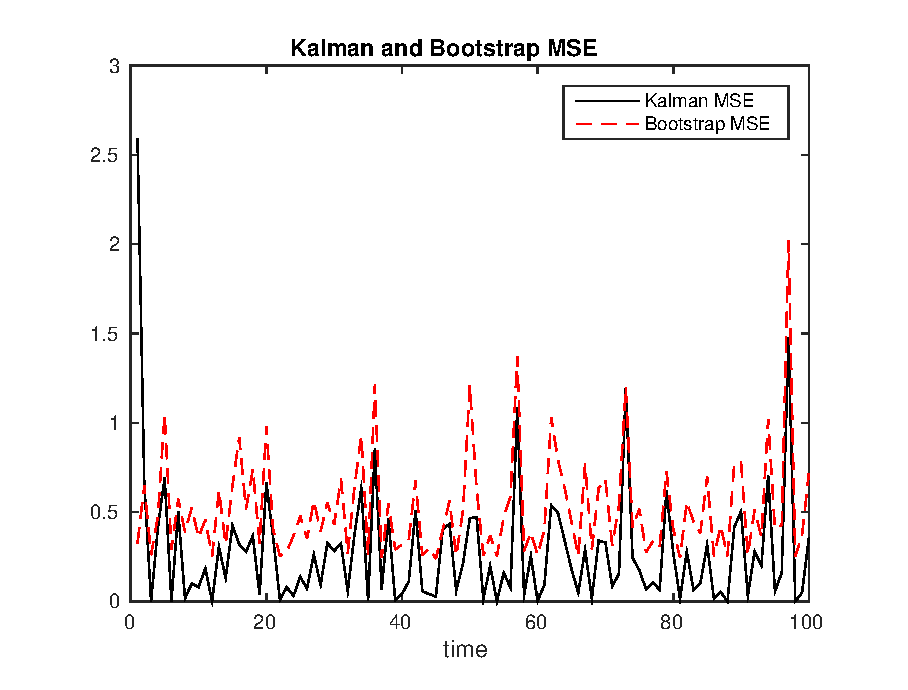
\includegraphics[width=80mm]{./kfigs/004_n5000MSE.eps}
    \caption{Mean square error for $N=5000$}
    \label{k3}
\end{figure}

\end{document}